\documentclass[11pt,a4paper]{article}
\usepackage[margin=0.75in]{geometry}
\usepackage{amsmath,amssymb}
\usepackage{tikz}
\usetikzlibrary{positioning,shapes,arrows,calc}
\usepackage{enumitem}
\usepackage{fancyhdr}
\usepackage{array}
\usepackage{booktabs}
\usepackage{hyperref}
\usepackage{tocloft}
\usepackage{xcolor}

\setlength{\headheight}{14pt}
\pagestyle{fancy}
\fancyhf{}
\fancyhead[L]{NMAM Institute of Technology, Nitte}
\fancyhead[R]{IV Semester B.E./B.Tech}
\fancyfoot[C]{\thepage}

\hypersetup{colorlinks=true,linkcolor=blue}

\newcommand{\examheader}[4]{
\noindent\rule{\textwidth}{0.5pt}\\
\textbf{#1} \hfill Duration: #3 | Max Marks: #4\\
\textbf{#2}\\
\rule{\textwidth}{0.5pt}
\vspace{0.2cm}
}

\begin{document}

% Title Page
\begin{titlepage}
\centering
\vspace*{2cm}
{\Huge\bfseries NMAM Institute of Technology, Nitte\par}
\vspace{0.5cm}
{\Large\itshape Off-Campus Centre of Nitte (Deemed to be University)\par}
\vspace{2cm}
{\Huge\bfseries COMPLETE EXAMINATION\\QUESTION BANK\par}
\vspace{1cm}
{\Large IV Semester B.E./B.Tech (CBCS)\par}
\vspace{1cm}
{\Large Academic Years: 2022--2025\par}
\vspace{2cm}
{\Large\bfseries Subjects:\par}
\vspace{0.5cm}
\begin{tabular}{|l|l|}
\hline
\textbf{Code} & \textbf{Subject} \\
\hline
MA2005-1 & Linear Algebra and Numerical Methods \\
CS2102-1 & Database Management Systems \\
CS3004-1 & Design and Analysis of Algorithms \\
CS2103-1 & Software Engineering \& Project Management \\
CS3005-1 & Microprocessor and Embedded Systems \\
ME1654-1 & Innovation and Design Thinking \\
\hline
\end{tabular}
\vfill
{\large Organized by: Subject $\to$ MSE-I $\to$ MSE-II $\to$ SEE\par}
\end{titlepage}

\tableofcontents
\newpage

%===============================================================================
\part{LINEAR ALGEBRA AND NUMERICAL METHODS}
%===============================================================================

%-------------------------------------------------------------------------------
\section{MSE-I Examinations}
%-------------------------------------------------------------------------------

\subsection{MA2005-1 MSE-I -- February 2025}
\examheader{Mid Semester Examination - I, February 2025}{MA2005-1 -- LINEAR ALGEBRA AND NUMERICAL METHODS}{1 Hour}{15}

\subsubsection*{Part A: Multiple Choice Questions (3 $\times$ 1 = 3 Marks)}

\begin{enumerate}
\item For what values of $k$ will the augmented matrix 
$\begin{bmatrix} 1 & 2 & 1 & | & 2 \\ 2 & 2 & 1 & | & 3 \\ 1 & 2 & k & | & k+1 \end{bmatrix}$
correspond to an inconsistent system of linear equations?

(A) $k \neq 1$ \quad (B) $k = 0$ \quad (C) $k = 1$ \quad (D) All values of $k$

\item If $A = \begin{bmatrix} 2 & 1 \\ 0 & 3 \end{bmatrix}$ and $B = \begin{bmatrix} 1 & 0 \\ 1 & 2 \end{bmatrix}$, find $(AB)^{-1}$.

(A) $\begin{bmatrix} 1 & 1/3 \\ -1/6 & 1/2 \end{bmatrix}$ \quad 
(B) $\begin{bmatrix} 1 & -1/2 \\ -1/6 & 1/2 \end{bmatrix}$ \quad 
(C) $\begin{bmatrix} 1 & -1/3 \\ -1/6 & 1/2 \end{bmatrix}$ \quad 
(D) $\begin{bmatrix} 1 & -1/3 \\ 1/6 & 1/2 \end{bmatrix}$

\item Given a matrix $A$, column 1 and column 3 are pivot columns, then the dimension of Col $A$ is:

(A) 1 \quad (B) 2 \quad (C) 3 \quad (D) 4
\end{enumerate}

\subsubsection*{Part B: Descriptive Questions (2 $\times$ 6 = 12 Marks)}

\textbf{UNIT -- I}

\textbf{Q1.} a) Find the eigenvalues of $A = \begin{bmatrix} 1 & 2 & 1 \\ 6 & -1 & 0 \\ -1 & -2 & -1 \end{bmatrix}$. Also determine the eigenvectors corresponding to each eigenvalue. \hfill [6 Marks]

b) Reduce the matrix $A = \begin{bmatrix} -2 & -4 & 2 \\ -2 & 1 & 2 \\ 4 & 2 & 5 \end{bmatrix}$ to the form $PA = LU$, using partial pivoting, where $L$ is a lower triangular matrix with unit diagonal entries and $U$ is an upper triangular matrix. \hfill [6 Marks]

\textbf{UNIT -- II}

\textbf{Q2.} a) Solve by Gauss-Seidel method: $10x + y + z = 12$; $2x + 10y + z = 13$; $x + y + 5z = 7$. (Perform 3 iterations) \hfill [6 Marks]

b) Find the dominant eigenvalue and corresponding eigenvector of $A = \begin{bmatrix} 1 & 6 & 1 \\ 1 & 2 & 0 \\ 0 & 0 & 3 \end{bmatrix}$ using Rayleigh's Power method (4 iterations). \hfill [6 Marks]

\vspace{0.5cm}
\hrule
\vspace{0.5cm}

\subsection{MA2005-1 MSE-I -- February 2024}
\examheader{Mid Semester Examination - I, February 2024}{MA2005-1 -- LINEAR ALGEBRA AND NUMERICAL METHODS}{1 Hour}{15}

\subsubsection*{Part B: Descriptive Questions}

\textbf{Q1.} a) Solve by Gauss-Seidel iteration method (4 iterations): $20x + y - 2z = 17$; $3x + 20y - z = -18$; $2x - 3y + 20z = 25$. Start with $x^{(0)} = y^{(0)} = z^{(0)} = 0$.

b) Using the power method, find the dominant eigenvalue and corresponding eigenvector of $A = \begin{bmatrix} 1 & -3 & 2 \\ 4 & 4 & -1 \\ 6 & 3 & 5 \end{bmatrix}$ starting with initial value $[1, 0, 0]^T$. (4 iterations)

\textbf{Q2.} a) Solve the system $x + y + z = 1$; $4x + 3y - z = 6$; $3x + 5y + 3z = 4$ by LU factorization method.

b) Find all eigenvalues of $A = \begin{bmatrix} 13 & -4 & 2 \\ -4 & 13 & -2 \\ 2 & -2 & 10 \end{bmatrix}$. Find eigenvector for largest eigenvalue.

\textbf{Q3.} a) Find the general solution of the system whose augmented matrix is $\begin{bmatrix} 1 & 3 & 4 & 7 \\ 3 & 9 & 7 & 6 \end{bmatrix}$.

b) Reduce the matrix $A = \begin{bmatrix} 0 & -3 & -6 & 4 & 9 \\ -1 & -2 & -1 & 3 & 1 \\ -2 & -3 & 0 & 3 & -1 \\ 1 & 4 & 5 & -9 & -7 \end{bmatrix}$ to echelon form and find its rank.

\vspace{0.5cm}
\hrule
\vspace{0.5cm}

\subsection{21CS401 MSE-I -- June 2023}
\examheader{Mid Semester Examination - I, June 2023}{21CS401 -- LINEAR ALGEBRA}{1 Hour}{20}

\subsubsection*{Part B: Descriptive Questions}

\textbf{Q1.} a) Find the eigenvalues and eigenvectors of the matrix.

b) Reduce the given matrix to echelon form.

\textbf{Q2.} a) Solve the system of equations using Gauss elimination method.

b) Solve using LU factorization method.

\textbf{Q3.} a) Apply Power method to find dominant eigenvalue (4 iterations).

b) Diagonalize the matrix $A = \begin{bmatrix} -1 & 2 \\ 2 & -1 \end{bmatrix}$. Hence find $A^6$.

%-------------------------------------------------------------------------------
\section{MSE-II Examinations}
%-------------------------------------------------------------------------------

\subsection{MA2005-1 MSE-II -- April 2025}
\examheader{Mid Semester Examination - II, April 2025}{MA2005-1 -- LINEAR ALGEBRA AND NUMERICAL METHODS}{1 Hour}{20}

\subsubsection*{Part A: Multiple Choice Questions (4 $\times$ 1 = 4 Marks)}

\begin{enumerate}
\item Let $T: \mathbb{R}^2 \to \mathbb{R}^2$ be a linear transformation such that $T(x_1, x_2) = (x_1 + x_2, x_1)$. Then $T^{-1}(x_1, x_2)$ equals:

(A) $(x_2, x_1 - x_2)$ \quad (B) $(x_2, x_1 + x_2)$ \quad (C) $(x_1, x_1 - x_2)$ \quad (D) $(x_1, x_1 + x_2)$

\item The set $\{1, x, x^2\}$ forms a basis for:

(A) $P_1$ \quad (B) $P_2$ \quad (C) $P_3$ \quad (D) $P_4$

\item Which of the following is a subspace of the given vector space?

(A) The set of all polynomials of degree exactly 3, in $P_3$\\
(B) The set of all polynomials with positive coefficients, in $P$\\
(C) The set of all $2 \times 2$ matrices with positive entries, in $M_{2 \times 2}$\\
(D) The set of all symmetric $2 \times 2$ matrices, in $M_{2 \times 2}$

\item Given matrix $A_{4 \times 5}$ with $\text{rank}(A) = 3$, then $\dim(\text{Null}(A))$ is:

(A) 1 \quad (B) 2 \quad (C) 3 \quad (D) 4
\end{enumerate}

\subsubsection*{Part B: Descriptive Questions (2 $\times$ 8 = 16 Marks)}

\textbf{UNIT -- I}

\textbf{Q1.} a) Let $T: P_2 \to P_2$ be the transformation that maps a polynomial $p(t)$ into the polynomial $p(t+2)$. Find the image of $p(t) = 3 - 2t + t^2$. Show that $T$ is a linear transformation. Find the matrix representation of $T$ relative to the basis $B = \{1, t, t^2\}$. \hfill [8 Marks]

b) Let $\vec{v_1} = (1, -2, 3)$, $\vec{v_2} = (5, 6, -1)$, $\vec{v_3} = (3, 2, 1)$. Show that the set $S = \{\vec{v_1}, \vec{v_2}, \vec{v_3}\}$ is a basis for $\mathbb{R}^3$. Express each of the standard basis vectors as linear combinations of the vectors in $S$. \hfill [8 Marks]

\textbf{UNIT -- II}

\textbf{Q2.} a) Use Gram-Schmidt process to construct orthonormal basis from the basis $B = \{(1,1,1), (0,1,1), (0,0,1)\}$ of $\mathbb{R}^3$. Find the QR factorization of the matrix whose column vectors form $B$. \hfill [8 Marks]

b) Use coordinate vectors to test the linear independence of the set of polynomials: $S = \{1 - 2t^2 - t^3, t + 2t^3, 1 + t - 2t^2\}$. \hfill [8 Marks]

\vspace{0.5cm}
\hrule
\vspace{0.5cm}

\subsection{21CS401 MSE-II -- July 2023}
\examheader{Mid Semester Examination - II, July 2023}{21CS401 -- LINEAR ALGEBRA}{1 Hour}{20}

\subsubsection*{Part A: Multiple Choice Questions (4 $\times$ 1 = 4 Marks)}

\begin{enumerate}
\item The dimension of the vector space of all symmetric $n \times n$ matrices is:

(A) $n^2$ \quad (B) $\frac{n(n+1)}{2}$ \quad (C) $\frac{n(n-1)}{2}$ \quad (D) $n$

\item Let $T: \mathbb{R}^2 \to \mathbb{R}^2$ be defined by $T(x,y) = (x+y, x-y)$. Then $T$ is:

(A) Linear but not one-to-one \quad (B) One-to-one but not onto\\
(C) Both one-to-one and onto \quad (D) Neither one-to-one nor onto

\item If $\{v_1, v_2, v_3\}$ is a basis for $V$, then $\{v_1 + v_2, v_2 + v_3, v_3 + v_1\}$ is:

(A) Always a basis \quad (B) Never a basis \quad (C) A basis if vectors are orthogonal \quad (D) Cannot be determined

\item The null space of an $m \times n$ matrix $A$ is a subspace of:

(A) $\mathbb{R}^m$ \quad (B) $\mathbb{R}^n$ \quad (C) $\mathbb{R}^{m+n}$ \quad (D) $\mathbb{R}^{mn}$
\end{enumerate}

\subsubsection*{Part B: Descriptive Questions (2 $\times$ 8 = 16 Marks)}

\textbf{Q1.} a) Let $V = P_2$ (polynomials of degree $\leq 2$). Show that $S = \{1+x, x+x^2, 1+x^2\}$ is a basis for $V$. \hfill [8 Marks]

b) Let $T: \mathbb{R}^3 \to \mathbb{R}^2$ be defined by $T(x,y,z) = (x+2y-z, 2x-y+z)$. Find the matrix of $T$ with respect to standard bases. Find $\ker(T)$ and $\text{range}(T)$. \hfill [8 Marks]

\textbf{Q2.} a) Use Gram-Schmidt process to orthonormalize the vectors $v_1 = (1,1,0)$, $v_2 = (1,0,1)$, $v_3 = (0,1,1)$. \hfill [8 Marks]

b) Find the least squares solution of $A\vec{x} = \vec{b}$ where $A = \begin{bmatrix} 1 & 1 \\ 1 & 2 \\ 1 & 3 \end{bmatrix}$, $\vec{b} = \begin{bmatrix} 1 \\ 2 \\ 4 \end{bmatrix}$. \hfill [8 Marks]

\vspace{0.5cm}
\hrule
\vspace{0.5cm}

\subsection{20CS401/20IS401/20AM401/20CC401 MSE-II -- June 2022}
\examheader{Mid Semester Examination - II, June 2022}{20CS401/20IS401/20AM401/20CC401 -- LINEAR ALGEBRA \& PROBABILITY THEORY}{1 Hour}{20}

\textit{Note: Answer any One full question from each Unit.}

\subsubsection*{UNIT -- I}

\textbf{Q1.} a) Check whether a transformation $T: \mathbb{R}^2 \to \mathbb{R}^3$ defined by $T(x,y) = (3x+y, 5x+7y, x+3y)$ is a linear transformation or not. \hfill [4 Marks]

b) State Rank-Nullity theorem. \hfill [4 Marks]

\textbf{Q2.} a) Let a linear transformation $T: \mathbb{R}^3 \to \mathbb{R}^3$ be defined by $T(x,y,z) = (x+2y-z, y+z, x+y-2z)$. Find the null space of $T$ and rank of $T$. \hfill [6 Marks]

\textbf{Q3.} Find the matrix of the linear transformation $T: \mathbb{R}^3 \to \mathbb{R}^2$ defined by $T(x,y,z) = (x-y+2z, 3x+y)$ with respect to bases $B = \{(1,1,1), (1,2,3), (1,0,0)\}$ and $B' = \{(1,1), (1,-1)\}$. \hfill [4 Marks]

\textbf{Q4.} Construct an orthonormal basis for a subspace $W$ of $\mathbb{R}^3$ with a basis $\{x_1, x_2, x_3\}$ where $x_1 = \begin{pmatrix} 1 \\ 0 \\ 1 \end{pmatrix}$, $x_2 = \begin{pmatrix} 1 \\ 0 \\ 0 \end{pmatrix}$, $x_3 = \begin{pmatrix} 2 \\ 1 \\ 0 \end{pmatrix}$ of $W$, using Gram-Schmidt process. \hfill [6 Marks]

\subsubsection*{UNIT -- II}

\textbf{Q5.} Find a least square solution of $AX = B$ where $A = \begin{bmatrix} 4 & 0 \\ 0 & 2 \\ 1 & 1 \end{bmatrix}$ and $B = \begin{bmatrix} 2 \\ 0 \\ 11 \end{bmatrix}$. \hfill [4 Marks]

\textbf{Q6.} a) The pdf $p(x)$ of a variate $X$ is given by the following table:

\begin{center}
\begin{tabular}{|c|c|c|c|c|c|c|c|}
\hline
$X$ & 0 & 1 & 3 & 4 & 5 & 6 \\
\hline
$p(x)$ & $k$ & $3k$ & $5k$ & $9k$ & $10k$ & $12k$ \\
\hline
\end{tabular}
\end{center}

For what value of $k$, does this represent a valid probability distribution? Also find $P(X > 3)$ and $E[X]$. \hfill [3+3 Marks]

b) If $f(x) = kx^3$, $0 < x < 1$, and $= 0$ elsewhere, is a pdf of the random variable $X$, find:
\begin{enumerate}[label=(\roman*)]
\item the value of $k$
\item $P(X > 0.7)$
\item $P\left(\frac{1/4 < X < 3/4}{X > 1/2}\right)$
\end{enumerate} \hfill [3+3 Marks]

\textbf{Q7.} a) If $X$ is a random variable, prove that:
\begin{enumerate}[label=(\roman*)]
\item $V(X) = E(X^2) - [E(X)]^2$
\item $V(aX + b) = a^2 V(X)$ where $a$ and $b$ are constants.
\end{enumerate} \hfill [4 Marks]

\textbf{Q8.} a) State Bayes' theorem. \hfill [2 Marks]

b) A business man goes to hotels $X$, $Y$, $Z$ 30\%, 45\% and 25\% of the time respectively. It is known that 5\%, 4\%, 6\% of the rooms in hotels $X$, $Y$, $Z$ respectively have faulty plumbing. Determine the probability:
\begin{enumerate}[label=(\roman*)]
\item that the business man goes to hotel with faulty plumbing
\item that business man's room having faulty plumbing is assigned to hotel $Y$?
\end{enumerate} \hfill [6 Marks]

%-------------------------------------------------------------------------------
\section{SEE (Semester End Examinations)}
%-------------------------------------------------------------------------------

\subsection{MA2005-1 SEE -- May 2025}
\examheader{Semester End Examination, May 2025}{MA2005-1 -- LINEAR ALGEBRA AND NUMERICAL METHODS}{3 Hours}{100}

\subsubsection*{Part A: Multiple Choice Questions (20 $\times$ 1 = 20 Marks)}

\begin{enumerate}
\item For what value of $k$, the augmented matrix $\begin{bmatrix} 1 & 3 & -2 & | & 3 \\ 3 & k & -6 & | & 9 \\ 1 & -3 & 2 & | & 5 \end{bmatrix}$ corresponds to an inconsistent system?

(A) $k = 1$ \quad (B) $k = 9$ \quad (C) $k = -3$ \quad (D) None of these

\item If $A$ and $B$ are two matrices such that $AB$ exists and is a square matrix, then:

(A) $A$ and $B$ are square matrices of same order\\
(B) Either both are square or number of rows of $A$ = number of columns of $B$\\
(C) $BA$ need not exist\\
(D) Any one of $A$ and $B$ is identity

\item Columns 1, 2 and 5 are pivot columns of a matrix $A$. Which is NOT necessarily true?

(A) $\dim(\text{Col } A) = 3$ \quad (B) $\dim(\text{Row } A) = 3$ \quad (C) $\text{rank}(A) = 3$ \quad (D) $\dim(\text{Null } A) = 3$

\item If $\lambda$ is an eigenvalue of $A$, then eigenvalue of $A^{-1}$ is:

(A) $\lambda$ \quad (B) $-\lambda$ \quad (C) $\lambda^2$ \quad (D) $1/\lambda$

\item If $A = \begin{bmatrix} 1 & 3 & 5 \\ 2 & 3 & 1 \\ 0 & 0 & 2 \end{bmatrix}$ then $A^3 - 3A^2 - A + 3I =$

(A) $A + I$ \quad (B) $I$ \quad (C) $2A$ \quad (D) $0$

\item The eigenvalues of $P^{-1}AP$ are:

(A) Same as that of $PA$ \quad (B) Same as that of $A$ \quad (C) Same as that of $P$ \quad (D) Cannot say

\item Correct order to solve by Gauss-Seidel method:

(A) Arrange in any order \quad (B) Diagonal elements are zero\\
(C) Diagonal elements larger than other elements \quad (D) Cannot be solved

\item Which is a direct method for solving system of linear equations?

(A) Jacobi \quad (B) Gauss-Seidel \quad (C) LU Decomposition \quad (D) Power method

\item If $\lambda$ is eigenvalue of $A$ with eigenvector $\vec{x}$, then $\lambda^2 + 1$ is eigenvalue of:

(A) $A^2 + I$ \quad (B) $A^2 + A$ \quad (C) $2A$ \quad (D) $(A + I)^2$

\item If $1 + x$, $1 + x + x^2$, and $ax^2 + x^3$ are linearly dependent, then $a =$:

(A) 1 \quad (B) 2 \quad (C) 3 \quad (D) 4

\item The dimension of subspace $W = \{(a, b, c, d) : a - 2b + c - d = 0\}$ is:

(A) 1 \quad (B) 2 \quad (C) 3 \quad (D) 4

\item Let $V$ be set of all $2 \times 2$ symmetric matrices. Then dimension of $V$ is:

(A) 1 \quad (B) 2 \quad (C) 3 \quad (D) 4

\item For linear transformation $T: V \to W$, let $U$ be subspace of $W$. Then $T^{-1}(U)$ is:

(A) Subspace of $V$ \quad (B) Subspace of $W$ \quad (C) Subspace of both \quad (D) Not a subspace

\item Every linear transformation $T: \mathbb{R}^n \to \mathbb{R}^m$ can be represented as matrix multiplication.

(A) True only if $m = n$ \quad (B) True only if $m \neq n$ \quad (C) Always true \quad (D) Never true

\item If $\vec{u}$ and $\vec{v}$ are orthogonal vectors in $\mathbb{R}^n$, then:

(A) $\|\vec{u} + \vec{v}\|^2 = \|\vec{u}\|^2 + \|\vec{v}\|^2$ \quad (B) $\|\vec{u} + \vec{v}\|^2 = \|\vec{u}\|^2 - \|\vec{v}\|^2$\\
(C) $\|\vec{u} + \vec{v}\|^2 = \|\vec{u}\|^2 \cdot \|\vec{v}\|^2$ \quad (D) $\|\vec{u} + \vec{v}\|^2 = \|\vec{u}\|^2 / \|\vec{v}\|^2$

\item Two vectors $\vec{u} = (1, 2, -3)$ and $\vec{v} = (a, 1, 1)$ are orthogonal if $a =$:

(A) 1 \quad (B) 2 \quad (C) 3 \quad (D) 5

\item A linear combination of the rows of $A$ can be written as:

(A) $\vec{x}^T A$ \quad (B) $A\vec{x}$ \quad (C) $\vec{x} A^T$ \quad (D) $A^T \vec{x}$

\item The angle between vectors $\vec{u} = (1, 2, -1, 0)$ and $\vec{v} = (-1, 1, 1, 2)$ is:

(A) $\pi/4$ \quad (B) $\pi/3$ \quad (C) $\pi/2$ \quad (D) $2\pi/3$

\item Which defines an inner product on $\mathbb{R}^2$?

(A) $\langle \vec{u}, \vec{v} \rangle = u_1 v_1 - u_2 v_2$ \quad (B) $\langle \vec{u}, \vec{v} \rangle = u_1 v_1 + 2u_2 v_2$\\
(C) $\langle \vec{u}, \vec{v} \rangle = u_1^2 v_1^2 + u_2^2 v_2^2$ \quad (D) $\langle \vec{u}, \vec{v} \rangle = u_1 v_2 - u_2 v_1$

\item For orthonormal basis $\{\vec{u}_1, \ldots, \vec{u}_n\}$ of $\mathbb{R}^n$ and any $\vec{x} \in \mathbb{R}^n$:

(A) $\|\vec{x}\|^2 = \sum_{i=1}^{n} |\langle \vec{x}, \vec{u}_i \rangle|^2$ \quad (B) $\|\vec{x}\|^2 = \sum_{i=1}^{n} \langle \vec{x}, \vec{u}_i \rangle$\\
(C) $\|\vec{x}\| = \sum_{i=1}^{n} |\langle \vec{x}, \vec{u}_i \rangle|$ \quad (D) None of the above
\end{enumerate}

\subsubsection*{Part B: Descriptive Questions (5 $\times$ 16 = 80 Marks)}

\textbf{UNIT -- I}

\textbf{Q1.} a) Find basis for Nul $A$ and Col $A$ where $A = \begin{bmatrix} 1 & 3 & 0 & 2 & -1 \\ 0 & 0 & 1 & -1 & 3 \\ 1 & 3 & 1 & 1 & 2 \\ -2 & -6 & 0 & -2 & 4 \end{bmatrix}$ \hfill [8 Marks]

b) Find eigenvalues of $A = \begin{bmatrix} 0 & -4 & -6 \\ -1 & 0 & -3 \\ 1 & 2 & 5 \end{bmatrix}$. Find eigenvectors and verify Cayley-Hamilton theorem. \hfill [8 Marks]

\textbf{Q2.} a) Compute $A^{10}$ if $A = \begin{bmatrix} 4 & -3 \\ 2 & -1 \end{bmatrix}$. \hfill [8 Marks]

b) Reduce $A = \begin{bmatrix} 2 & 1 & 1 \\ 4 & -6 & 0 \\ -2 & 7 & 2 \end{bmatrix}$ to $A = LU$. Use factorization to solve $A\vec{x} = \vec{b}$ where $\vec{b} = \begin{bmatrix} 1 \\ -2 \\ 3 \end{bmatrix}$. \hfill [8 Marks]

\textbf{UNIT -- II}

\textbf{Q3.} a) Solve by Gauss-Seidel method (4 iterations): $10x - y + 2z = 6$; $-x + 11y - z + 3w = 25$; $2x - y + 10z - w = -11$; $3y - z + 8w = 15$. \hfill [8 Marks]

b) Find dominant eigenvalue and eigenvector of $A = \begin{bmatrix} 2 & -1 & 0 \\ -1 & 2 & -1 \\ 0 & -1 & 2 \end{bmatrix}$ using Power method (5 iterations). \hfill [8 Marks]

\textbf{Q4.} a) Let $V = M_{2 \times 2}$. Show $W = \left\{ \begin{bmatrix} a & b \\ c & d \end{bmatrix} : a + d = 0 \right\}$ is subspace of $V$. Find its dimension. \hfill [8 Marks]

b) Let $T: \mathbb{R}^2 \to \mathbb{R}^3$ be $T(x_1, x_2) = (x_1 - x_2, x_1, 2x_1 + x_2)$. Show $T$ is linear. Find matrix. Is $T$ one-to-one? Is $T$ onto? \hfill [8 Marks]

\textbf{UNIT -- III}

\textbf{Q5.} a) Find QR factorization of $A = \begin{bmatrix} 1 & -1 & 4 \\ 1 & 4 & -2 \\ 1 & 4 & 2 \\ 1 & -1 & 0 \end{bmatrix}$. \hfill [8 Marks]

b) For $A = \begin{bmatrix} 4 & 11 & 14 \\ 8 & 7 & -2 \end{bmatrix}$, find the SVD of $A$. \hfill [8 Marks]

\textbf{Q6.} a) Find best line $y = \beta_0 + \beta_1 x$ for data points: $(0, 1), (1, 1), (2, 2), (3, 2)$ using least squares. \hfill [8 Marks]

b) Let $S = \{(2, 5, -3, -1), (-2, -3, 2, -5), (1, 3, -2, 0), (-1, -6, 3, 3)\}$. Find basis for subspace of $\mathbb{R}^4$ spanned by $S$. \hfill [8 Marks]

\newpage
%===============================================================================
\part{DATABASE MANAGEMENT SYSTEMS}
%===============================================================================

%-------------------------------------------------------------------------------
\section{MSE-I Examinations}
%-------------------------------------------------------------------------------

\subsection{CS2102-1 MSE-I -- February 2025}
\examheader{Mid Semester Examination - I, February 2025}{CS2102-1 -- DATABASE MANAGEMENT SYSTEMS}{1 Hour}{15}

\subsubsection*{Part A: Multiple Choice Questions (3 $\times$ 1 = 3 Marks)}

\begin{enumerate}
\item A \_\_\_\_\_\_ is a unit of storage containing one or more records.

(A) Block \quad (B) Field \quad (C) Tuple \quad (D) File

\item Which of the following is NOT a component of ER Model?

(A) Entity \quad (B) Attribute \quad (C) Table \quad (D) Relationship

\item Which of the following is used to uniquely identify a record in a table?

(A) Foreign Key \quad (B) Candidate Key \quad (C) Primary Key \quad (D) Super Key
\end{enumerate}

\subsubsection*{Part B: Descriptive Questions (2 $\times$ 6 = 12 Marks)}

\textbf{UNIT -- I}

\textbf{Q1.} a) Design and construct an ER diagram for ``Student Database Management System''. Indicate all keys, constraints and assumptions. \hfill [6 Marks]

b) Discuss the main characteristics of the database approach. \hfill [6 Marks]

\textbf{Q2.} a) Identify the Entity, Relationship, Participation Constraint and Cardinality ratio for the ER diagram of Movie database schema (ACTOR, MOVIE, DIRECTOR, PRODUCER entities with relationships). \hfill [6 Marks]

b) Describe Three Schema Architecture with a neat diagram. \hfill [6 Marks]

\textbf{UNIT -- II}

\textbf{Q3.} a) Write the following queries in Relational Algebra for:
\begin{verbatim}
EMPLOYEE(SSN, SNAME, AGE, SALARY, DEPT_ID)
DEPARTMENT(DEPT_ID, DEPT_NAME, DEPT_HEAD)
PROJECT(PID, DEPT_ID, PNAME)
WORKSON(SSN, PID, PHOURS)
\end{verbatim}
(i) Get names of employees working on projects managed by 'HR' department.\\
(ii) Retrieve names of employees who do not work on any project.\\
(iii) Find names of all departments that have at least one project. \hfill [6 Marks]

b) Explain how to deal with constraints violation during insertion and delete operations. \hfill [6 Marks]

\vspace{0.5cm}
\hrule
\vspace{0.5cm}

\subsection{CS2102-1 MSE-I -- February 2024}
\examheader{Mid Semester Examination - I, February 2024}{CS2102-1 -- DATABASE MANAGEMENT SYSTEMS}{1 Hour}{15}

\subsubsection*{Part B: Descriptive Questions}

\textbf{Q1.} a) Describe Three Schema Architecture with diagram. Why do we need mappings among schema levels? \hfill [6 Marks]

b) Design ER diagram for ``Engineering College Management System''. \hfill [6 Marks]

\textbf{Q2.} a) Discuss the main characteristics of database approach. \hfill [6 Marks]

b) Explain domain constraints and referential integrity constraints in relational model. \hfill [6 Marks]

\textbf{Q3.} a) Define Entity attribute. Explain different types of attributes in ER diagram. \hfill [6 Marks]

b) Outline steps to convert basic ER model to relational database scheme. \hfill [6 Marks]

\textbf{Q4.} a) ``For good database design, matching attributes must be primary key or foreign key otherwise it leads to spurious tuples''. Justify. \hfill [6 Marks]

b) Discuss the characteristics of relations. \hfill [6 Marks]

%-------------------------------------------------------------------------------
\section{MSE-II Examinations}
%-------------------------------------------------------------------------------

\subsection{CS2102-1 MSE-II -- April 2025}
\examheader{Mid Semester Examination - II, April 2025}{CS2102-1 -- DATABASE MANAGEMENT SYSTEMS}{1 Hour}{20}

\subsubsection*{Part A: Multiple Choice Questions (4 $\times$ 1 = 4 Marks)}

\begin{enumerate}
\item The rule ``No component of Primary Key accepts Null value'' is:

(A) Referential Integrity Constraint \quad (B) Domain Integrity Constraint\\
(C) Entity Integrity Constraint \quad (D) Tuple Integrity Constraint

\item Which command adds a new column to existing table?

(A) ALTER \quad (B) UPDATE \quad (C) INSERT \quad (D) MODIFY

\item A relation is in BCNF if every non-trivial FD $X \to Y$:

(A) $X$ is a super key \quad (B) $Y$ is a prime attribute\\
(C) $X$ is a candidate key \quad (D) $Y$ is a super key

\item The operation to combine tuples from two relations based on condition:

(A) Union \quad (B) Join \quad (C) Projection \quad (D) Selection
\end{enumerate}

\subsubsection*{Part B: Descriptive Questions (2 $\times$ 8 = 16 Marks)}

\textbf{Q1.} Consider the schema and write SQL queries:
\begin{verbatim}
Suppliers(sid: integer, sname: string, address: string)
Parts(pid: integer, pname: string, color: string)
Catalog(sid: integer, pid: integer, cost: double)
\end{verbatim}

(i) Find the sids of suppliers who supply some red or green part.\\
(ii) Find the sids of suppliers who supply only red parts.\\
(iii) Find the pnames of parts for which there is some supplier.\\
(iv) Find the sids of suppliers who supply some red part or are at 221 Packer Street. (Nested Query) \hfill [8 Marks]

\textbf{Q2.} Consider the schema and write SQL queries:
\begin{verbatim}
Movie(movie_id, title, release_year, genre, director_id, rating)
Director(director_id, name, birth_year, nationality)
Actor(actor_id, name, birth_year, nationality)
Movie_Actor(movie_id, actor_id, role)
Review(rev_id, user_id, movie_id, rev_text, rating, rev_date)
User(user_id, username, email, age)
\end{verbatim}

(i) Find names of actors who acted in at least one movie released after 2015.\\
(ii) Find directors who directed more than 5 movies.\\
(iii) Get average rating of movies directed by 'Christopher Nolan'.\\
(iv) Find movies with higher rating than average rating of same genre. (Nested Query) \hfill [8 Marks]

\textbf{Q3.} a) Consider FDs $F = \{A \to C, AC \to D, E \to AD, E \to H\}$ and $G = \{A \to CD, E \to AH\}$. Are they equivalent? \hfill [8 Marks]

b) What is Normalization? Explain First Normal Form with example. \hfill [8 Marks]

\textbf{Q4.} a) Given $R(ABCDEFGHIJ)$ and FDs: $\{(A,B) \to C, A \to \{D,E\}, B \to F, F \to \{G,H\}, D \to \{I,J\}\}$. Find candidate key. Check if relation is in 3NF. If not, decompose to 3NF. \hfill [8 Marks]

b) Explain any two Informal Design Guidelines for Relation Schemas. \hfill [8 Marks]

%-------------------------------------------------------------------------------
\section{SEE (Semester End Examinations)}
%-------------------------------------------------------------------------------

\subsection{CS2102-1 SEE -- May 2025}
\examheader{Semester End Examination, May 2025}{CS2102-1 -- DATABASE MANAGEMENT SYSTEMS}{3 Hours}{100}

\subsubsection*{Part A: Multiple Choice Questions (20 $\times$ 1 = 20 Marks)}

\begin{enumerate}
\item Which is not a characteristic of DBMS? (A) Data Independence (B) Concurrent Access (C) Data Redundancy (D) Data Security

\item Weak entity is represented by: (A) Rectangle (B) Double Rectangle (C) Diamond (D) Oval

\item Grouping related objects in ER model: (A) Aggregation (B) Generalization (C) Specialization (D) Composition

\item Each row of table represents a: (A) Field (B) Record (C) Attribute (D) Key

\item Retrieve data from multiple tables: (A) Union (B) Intersection (C) Cartesian Product (D) Projection

\item Produces relation with only specified attributes: (A) Selection (B) Projection (C) Join (D) Division

\item Filter groups formed by GROUP BY: (A) WHERE (B) ORDER BY (C) HAVING (D) FILTER

\item NOT a DML command: (A) SELECT (B) INSERT (C) CREATE (D) UPDATE

\item Trivial FD $X \to Y$ if: (A) $X \subseteq Y$ (B) $Y \subseteq X$ (C) $X = Y$ (D) $X \cap Y = \phi$

\item Eliminates transitive dependencies: (A) 1NF (B) 2NF (C) 3NF (D) BCNF

\item Closure of attributes $X$ under FDs $F$: (A) $X^+$ (B) $F^+$ (C) $X^*$ (D) $F^*$

\item 2NF requires 1NF and: (A) No partial dependencies (B) No transitive dependencies (C) Every determinant is candidate key (D) All attributes atomic

\item Lossless join decomposition uses: (A) Union (B) Intersection (C) Natural join (D) Cartesian product

\item NOT property of good decomposition: (A) Lossless join (B) Dependency preservation (C) Redundancy (D) No anomalies

\item Minimal cover has: (A) Single attribute on RHS (B) No redundant FDs (C) No extraneous attributes on LHS (D) All of the above

\item Permanently save transaction changes: (A) SAVEPOINT (B) COMMIT (C) ROLLBACK (D) GRANT

\item ACID properties include: (A) Atomicity, Consistency, Isolation, Durability (B) Atomicity, Concurrency, Isolation, Durability (C) Accuracy, Consistency, Integrity, Durability (D) Atomicity, Consistency, Integrity, Durability

\item Conflict serializable if: (A) Can transform to serial schedule by swapping non-conflicting operations (B) All transactions execute serially (C) No conflicts (D) Precedence graph has no cycles

\item Guarantees deadlock freedom: (A) Simple Lock (B) Two-Phase Locking (C) Strict 2PL (D) Wait-Die Scheme

\item Timestamp ordering for write on $X$: (A) Always allowed (B) If $TS > W\text{-timestamp}(X)$ and $TS > R\text{-timestamp}(X)$ (C) If $TS < W\text{-timestamp}(X)$ (D) Never allowed
\end{enumerate}

\subsubsection*{Part B: Descriptive Questions (80 Marks)}

\textbf{Q1.} a) What are Characteristics of Database approach? Explain. \hfill [8 Marks]

b) With neat diagram, explain Three Schema architecture. \hfill [8 Marks]

\textbf{Q2.} a) Explain attribute types: (i) Composite (ii) Multivalued (iii) Atomic. \hfill [8 Marks]

b) Explain Cardinality Ratio for Binary relationships with examples. \hfill [8 Marks]

\textbf{Q3.} a) Consider STUDENT and COURSE tables. Write Relational Algebra queries. \hfill [8 Marks]

b) Explain steps in ER to Relational Mapping Algorithm. \hfill [8 Marks]

\textbf{Q4.} a) Explain Not Null, DEFAULT and CHECK constraints in SQL. \hfill [8 Marks]

b) Explain CASCADE and RESTRICT options of DROP TABLE. \hfill [8 Marks]

\textbf{Q5.} a) What are Informal Design Guidelines for relational schema? \hfill [8 Marks]

b) What is Functional Dependency? Explain with example. \hfill [8 Marks]

\textbf{Q6.} a) Explain Standard Inference rules for Functional Dependencies. \hfill [8 Marks]

b) Explain algorithm for determining $X^+$, Closure of $X$ under $F$. \hfill [8 Marks]

\textbf{Q7.} a) What is B+ Tree? Explain structure \& characteristics with diagram. \hfill [8 Marks]

b) Briefly explain ACID properties. \hfill [8 Marks]

\textbf{Q8.} a) What is Query Optimizer? Explain working with diagram. \hfill [8 Marks]

b) What are 2 rules of Strict 2PL? Explain. \hfill [8 Marks]

\vspace{0.5cm}
\hrule
\vspace{0.5cm}

\subsection{CS2102-1 SEE -- July 2024}
\examheader{Semester End Examination, July 2024}{CS2102-1 -- DATABASE MANAGEMENT SYSTEMS}{3 Hours}{100}

\subsubsection*{Part B: Descriptive Questions}

\textbf{Q1.} a) Briefly explain various characteristics of database approach. \hfill [8 Marks]

b) Explain Relational Algebra operations: (i) Division (ii) Union (iii) Cartesian product (iv) COUNT. \hfill [8 Marks]

\textbf{Q2.} a) Design ER diagram and schema for flight management system. \hfill [8 Marks]

b) Explain grouping concepts in relational algebra. \hfill [8 Marks]

\textbf{Q3.} a) With block diagram explain three schema architecture. \hfill [8 Marks]

b) Sailors-Boats-Reserves queries in Relational Algebra. \hfill [8 Marks]

\textbf{Q4.} a) Employee-Works-Company-Manages SQL queries. \hfill [8 Marks]

b) What is a view? Give specification in SQL. \hfill [8 Marks]

\textbf{Q5.} a) Check lossless join property for given decompositions. \hfill [8 Marks]

b) How basic constraints are specified in SQL-99. \hfill [8 Marks]

\textbf{Q6.} a) Order processing database SQL queries. \hfill [8 Marks]

b) Need for normalization. Explain 1NF, 2NF, 3NF with examples. \hfill [8 Marks]

\textbf{Q7.} a) Explain Strict Two-Phase Locking protocol. \hfill [8 Marks]

b) Explain index structures: Hash based, Tree based indexing. \hfill [8 Marks]

\textbf{Q8.} a) Illustrate anomalies with Interleaved Execution. \hfill [8 Marks]

b) Algorithm to insert element in B+ tree. \hfill [8 Marks]

\newpage
%===============================================================================
\part{DESIGN AND ANALYSIS OF ALGORITHMS}
%===============================================================================

%-------------------------------------------------------------------------------
\section{MSE-I Examinations}
%-------------------------------------------------------------------------------

\subsection{CS3004-1 MSE-I -- February 2025}
\examheader{Mid Semester Examination - I, February 2025}{CS3004-1 -- DESIGN AND ANALYSIS OF ALGORITHMS}{1 Hour}{15}

\subsubsection*{Part A: Multiple Choice Questions (3 $\times$ 1 = 3 Marks)}

\begin{enumerate}
\item If algorithm has $T(n) = 7n^3 + 10n^2 + 4$, then $T(n)$ belongs to:

(A) $O(n)$ \quad (B) $O(n^2)$ \quad (C) $O(n^3)$ \quad (D) $O(n^4)$

\item Time complexity of $T(n) = 2T(n/2) + n$:

(A) $O(n)$ \quad (B) $O(n \log n)$ \quad (C) $O(n^2)$ \quad (D) $O(\log n)$

\item Minimum comparisons to find minimum in array of $n$ elements:

(A) $n$ \quad (B) $n - 1$ \quad (C) $n + 1$ \quad (D) $2n$
\end{enumerate}

\subsubsection*{Part B: Descriptive Questions (2 $\times$ 6 = 12 Marks)}

\textbf{UNIT -- I}

\textbf{Q1.} a) Summarize algorithm design and analysis process with diagram. \hfill [6 Marks]

b) For given algorithm, determine: (i) What it computes (ii) Basic operation (iii) How many times executed (iv) Efficiency. \hfill [6 Marks]

\textbf{Q2.} a) Define asymptotic notations Big Oh ($O$) and Big Theta ($\Theta$) with examples. \hfill [6 Marks]

b) Show that efficiency of Tower of Hanoi is exponential. \hfill [6 Marks]

\textbf{UNIT -- II}

\textbf{Q3.} a) Develop brute force string matching algorithm. Analyze worst-case complexity. \hfill [6 Marks]

b) Outline merge sort algorithm and derive time complexity. \hfill [6 Marks]

\textbf{Q4.} a) Define TSP. Solve using exhaustive search for 4-vertex graph with edges: A-B=6, A-C=3, A-D=1, B-C=4, B-D=2, C-D=8. State efficiency. \hfill [6 Marks]

b) Apply Quick sort on marks: 8, 10, 5, 2, 14. Show tree of recursive calls. \hfill [6 Marks]

\vspace{0.5cm}
\hrule
\vspace{0.5cm}

\subsection{CS3004-1 MSE-I -- February 2024}
\examheader{Mid Semester Examination - I, February 2024}{CS3004-1 -- DESIGN AND ANALYSIS OF ALGORITHMS}{1 Hour}{15}

\subsubsection*{Part B: Descriptive Questions}

\textbf{Q1.} a) Explain properties of algorithm using linear search example. \hfill [6 Marks]

b) For each function, indicate change when argument increased fourfold: (i) $\log_2 n$ (ii) $n$ (iii) $n^2$ (iv) $2^n$ (v) $\sqrt{n}$. \hfill [6 Marks]

\textbf{Q2.} a) Explain general framework for Analysis of an algorithm. \hfill [6 Marks]

b) Define 3 asymptotic notations. Check: (i) $10n^2 + 9 \in O(n^2)$ (ii) $n(n+1)/2 \in O(n^2)$. \hfill [6 Marks]

\textbf{Q3.} a) Write general plan for analyzing recursive algorithm. Find factorial efficiency. \hfill [6 Marks]

b) Give two brute force algorithms to sort integers. \hfill [6 Marks]

\textbf{Q4.} a) Illustrate Merge sort and analyze efficiency. Sort: 6, 14, 8, 2, 15, 10, 7, 5. \hfill [6 Marks]

b) Show comparisons for brute force string matching: P=0001 in T=000010001010101. \hfill [6 Marks]

\vspace{0.5cm}
\hrule
\vspace{0.5cm}

\subsection{21CS402 MSE-I -- June 2023}
\examheader{Mid Semester Examination - I, June 2023}{21CS402 -- DESIGN AND ANALYSIS OF ALGORITHMS}{1 Hour}{20}

\subsubsection*{Part B: Descriptive Questions}

\textbf{Q1.} a) With process flow diagram explain algorithm design and analysis. \hfill [8 Marks]

b) Design recursive algorithm for $2^n = 2^{n-1} + 2^{n-1}$. Find complexity. \hfill [8 Marks]

\textbf{Q2.} a) Define three asymptotic notations. Express $f(n) = n(n-1)/2$ using three notations with proof. \hfill [8 Marks]

b) Perform complexity analysis of sequential search for three efficiency types. \hfill [8 Marks]

\textbf{Q3.} a) What is brute force? Give brute force string matching with complexity. Trace: TEXT: JIM SAW ME IN SHOE SHOP, PATTERN: SHE. \hfill [8 Marks]

b) Apply merge sort to L,A,S,T,S,O,R,T,I,N,G alphabetically. Analyze complexity. \hfill [8 Marks]

\textbf{Q4.} a) Give complete Quick sort algorithm with complexity analysis. Trace for: 5, 3, 1, 9, 8, 2, 4, 7. \hfill [8 Marks]

b) What is exhaustive search? Solve knapsack: $n=4$, capacity $m=10$, $w=(4,6,3,5)$, values $=(30,50,20,10)$. \hfill [8 Marks]

%-------------------------------------------------------------------------------
\section{MSE-II Examinations}
%-------------------------------------------------------------------------------

\subsection{CS3004-1 MSE-II -- April 2025}
\examheader{Mid Semester Examination - II, April 2025}{CS3004-1 -- DESIGN AND ANALYSIS OF ALGORITHMS}{1 Hour}{20}

\subsubsection*{Part A: Multiple Choice Questions (4 $\times$ 1 = 4 Marks)}

\begin{enumerate}
\item Necessary condition for topological sorting:

(A) Graph must be tree \quad (B) Graph must be DAG\\
(C) Graph must be complete \quad (D) Graph must be bipartite

\item Data structure used in DFS:

(A) Queue \quad (B) Heap \quad (C) Priority queue \quad (D) Stack

\item Time complexity of distribution counting sort:

(A) $\Theta(n^2)$ \quad (B) $O(n \log n)$ \quad (C) $O(2^n)$ \quad (D) $\Theta(n)$

\item Dynamic programming builds solution from:

(A) Overlapping subproblems \quad (B) Single recursive call\\
(C) Greedy approach \quad (D) Divide and conquer
\end{enumerate}

\subsubsection*{Part B: Descriptive Questions (2 $\times$ 8 = 16 Marks)}

\textbf{Q1.} a) Outline Insertion sort algorithm. Show sorting of E, X, A, M, P, L, E in alphabetical order. \hfill [4 Marks]

b) Apply heap sort to: 90, 89, 56, 72, 67, 12, 21, 34, 45. \hfill [4 Marks]

\textbf{Q2.} a) Define AVL tree. Construct AVL tree for $\{2, 9, 3, 12, 15, 8, 11\}$. \hfill [4 Marks]

b) Define topological sorting. Illustrate using Source Removal method for given graph. \hfill [4 Marks]

\textbf{Q3.} a) Write Comparison Counting sort algorithm. Compare complexity with Selection and Bubble sort. \hfill [4 Marks]

b) Summarize Horspool algorithm. Search TIME in ``A STITCH IN TIME SAVES NINE''. \hfill [4 Marks]

\textbf{Q4.} a) Apply All Pair Shortest Path algorithm for given weighted graph. \hfill [4 Marks]

b) Write BFS algorithm. List two facts differentiating BFS from DFS. \hfill [4 Marks]

\vspace{0.5cm}
\hrule
\vspace{0.5cm}

\subsection{20CS402/20IS402/20AM402/20CC402 MSE-II -- June 2022}
\examheader{Mid Semester Examination - II, June 2022}{20CS402/20IS402/20AM402/20CC402 -- DESIGN AND ANALYSIS OF ALGORITHMS}{1 Hour}{20}

\textit{Note: Answer any One full question from each Unit.}

\subsubsection*{UNIT -- I}

\textbf{Q1.} Develop an algorithm to perform Insertion Sort and analyze the best and worst case efficiencies. \hfill [4 Marks]

\textbf{Q2.} Find the solution for following problem using topological sorting method. Consider a set of 5 courses $\{C_1, C_2, C_3, C_4, C_5\}$, a part time student has to take in some degree program. The courses can be taken in any order as long as the following course prerequisites are met: $C_1$ and $C_2$ have no prerequisites, $C_3$ requires $C_1$ and $C_2$, $C_4$ requires $C_3$ and $C_5$ requires $C_3$ and $C_4$. The student can take only one course per term. \hfill [3 Marks]

\textbf{Q3.} Construct 2-3 tree for the data: C, O, M, P, U, T, I, N, G. \hfill [3 Marks]

\textbf{Q4.} Explain Horspool's algorithm and apply the algorithm to find the pattern ``MONEY'' in the text ``A FOOL AND HIS MONEY ARE PARTED SOON''. \hfill [4 Marks]

\textbf{Q5.} Apply closed hashing to distribute the keys 10, 23, 14, 19, 17, 32, 45 using the function $H(k) = K \mod 11$. \hfill [2 Marks]

\textbf{Q6.} Construct heap and sort using array representation: 2, 9, 8, 14, 22, 16, 7. \hfill [4 Marks]

\subsubsection*{UNIT -- II}

\textbf{Q7.} Outline the pseudocode for Prim's algorithm to find the minimum spanning tree. Apply the Prim's algorithm to find the minimum spanning tree for the following graph:

\begin{center}
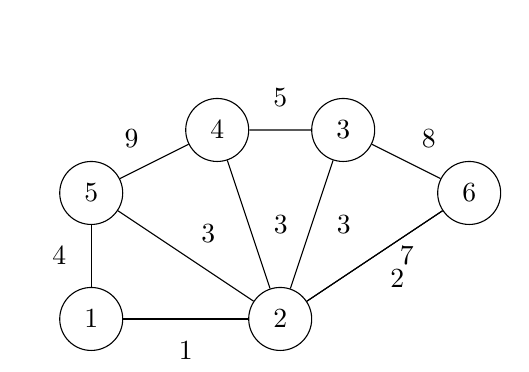
\begin{tikzpicture}[scale=0.8, every node/.style={circle, draw, minimum size=0.8cm}]
\node (5) at (0,2) {5};
\node (4) at (2,3) {4};
\node (3) at (4,3) {3};
\node (6) at (6,2) {6};
\node (1) at (0,0) {1};
\node (2) at (3,0) {2};
\draw (5) -- node[above left, draw=none] {9} (4);
\draw (4) -- node[above, draw=none] {5} (3);
\draw (3) -- node[above right, draw=none] {8} (6);
\draw (5) -- node[left, draw=none] {4} (1);
\draw (1) -- node[below, draw=none] {1} (2);
\draw (2) -- node[below right, draw=none] {2} (6);
\draw (4) -- node[right, draw=none] {3} (2);
\draw (3) -- node[right, draw=none] {3} (2);
\draw (5) -- node[above right, draw=none] {3} (2);
\draw (2) -- node[right, draw=none] {7} (6);
\end{tikzpicture}
\end{center}
\hfill [6 Marks]

\textbf{Q8.} Write a pseudocode for Bellman Ford algorithm to find the single source shortest path. \hfill [4 Marks]

\textbf{Q9.} a) Construct a Huffman code for the following data:

\begin{center}
\begin{tabular}{|c|c|c|c|c|c|}
\hline
Character & A & B & C & D & \_ \\
\hline
Probability & 0.4 & 0.1 & 0.2 & 0.15 & 0.15 \\
\hline
\end{tabular}
\end{center}

Encode the text ``ABACABAD'' using the code obtained. Decode the text whose encoding is 1000101110010010. \hfill [6 Marks]

b) Write the pseudocode for single source shortest path in DAG. \hfill [4 Marks]

%-------------------------------------------------------------------------------
\section{SEE (Semester End Examinations)}
%-------------------------------------------------------------------------------

\subsection{CS3004-1 SEE -- May 2025}
\examheader{Semester End Examination, May 2025}{CS3004-1 -- DESIGN AND ANALYSIS OF ALGORITHMS}{3 Hours}{100}

\subsubsection*{Part A: Multiple Choice Questions (20 $\times$ 1 = 20 Marks)}

\begin{enumerate}
\item Quick sort divides array into: (A) One (B) Two (C) Three (D) Four

\item Binary Search works on: (A) Unsorted (B) Sorted (C) Distinct elements (D) Integers only

\item Linear search is also called: (A) Binary search (B) Simple search (C) Sequential search (D) Difficult search

\item $O(n)$ means: (A) Exponential (B) Linear growth (C) Independent of input (D) Logarithmic

\item Output of fun(5) where fun(n) returns 1 if n==1, else n+fun(n-1): (A) 120 (B) 24 (C) 6 (D) 15

\item Pseudocode uses: (A) Native + programming language (B) High level only (C) Natural language only (D) Low level

\item NOT a characteristic of good algorithm: (A) Clarity (B) Efficiency (C) Correctness (D) Complex data structures

\item Primary characteristic of Divide and Conquer: (A) Iteration (B) Overlapping subproblems (C) Dividing into independent subproblems, solving recursively, combining (D) Linear solving

\item 0/1 Knapsack uses: (A) Greedy (B) Divide and conquer (C) Dynamic programming (D) DFS

\item Floyd-Warshall finds: (A) Shortest path between two nodes (B) Shortest paths between all pairs (C) Longest path (D) Pattern matching

\item Horspool uses which table: (A) Shift Table (B) Hash Table (C) Match Table (D) Character Table

\item Counting Sort is distribution-based because: (A) Uses frequencies for positions (B) Divides into subarrays (C) Compares pairs (D) Recursively splits

\item Max-heap root from [3, 9, 2, 1, 4, 8]: (A) 1 (B) 9 (C) 2 (D) 8

\item AVL rotation when balance factor $>1$ or $<-1$: (A) Rotation (B) Deletion (C) Insertion (D) Search

\item Binary Search is: (A) Decrease by constant (B) Decrease by constant factor (C) Decrease by one (D) Divide and conquer

\item In max-heap: (A) Parent smaller (B) Parent greater or equal (C) BST (D) Ascending order

\item Job Assignment minimizes: (A) Time (B) Number of tasks (C) Total cost (D) Total time worked

\item Subset-sum backtracks when: (A) Sum exceeds target (B) Sum equals target (C) All elements considered (D) Subset found

\item Dijkstra's Algorithm is: (A) Greedy (B) Branch and bound (C) Backtracking (D) Dynamic programming

\item Huffman codes use: (A) Exhaustive search (B) Greedy (C) Brute force (D) Divide and conquer
\end{enumerate}

\subsubsection*{Part B: Descriptive Questions (80 Marks)}

\textbf{UNIT -- I}

\textbf{Q1.} a) Explain Performance Analysis of algorithm. \hfill [8 Marks]

b) Write Selection sort pseudocode and analyze. Sort: 5, 4, 2, 1, 6, 3. \hfill [8 Marks]

\textbf{Q2.} a) General plan for non-recursive algorithm analysis. Find maximal element and analyze. \hfill [8 Marks]

b) Write Merge sort algorithm. Derive time complexity using recurrence. Sort: 38, 27, 43, 3, 9, 82, 10. \hfill [8 Marks]

\textbf{UNIT -- II}

\textbf{Q3.} a) Write insertion sort. Construct heap for: 63, 9, 19, 7, 90, 81, 45. \hfill [8 Marks]

b) Identify ``JIM\_SAM'' using Horspool in ``JIM\_SAW\_ME\_IN\_A\_BARBERSHOP''. \hfill [8 Marks]

\textbf{Q4.} a) Write B-Tree insertion algorithm. Draw B-Tree of order 5 for: 3, 14, 7, 1, 8, 5, 11, 17, 13, 6, 23, 12, 20, 26, 4, 16, 18, 24, 25, 19. \hfill [8 Marks]

b) Define Topological Sorting. Illustrate using source removal method. \hfill [8 Marks]

\textbf{UNIT -- III}

\textbf{Q5.} a) Write Divide and Conquer algorithm for key comparisons. Derive complexity. Quick sort: 38, 27, 43, 3, 9, 82, 10. \hfill [8 Marks]

b) Define Class P, Class NP, NP-Complete, NP-Hard. \hfill [8 Marks]

\textbf{Q6.} a) Solve Job assignment using Branch and Bound for matrix:
$\begin{bmatrix} 9 & 2 & 7 & 8 \\ 6 & 4 & 3 & 7 \\ 5 & 8 & 1 & 8 \\ 7 & 6 & 9 & 4 \end{bmatrix}$ \hfill [8 Marks]

b) Solve subset sum using backtracking: $S = \{5, 10, 12, 13, 15, 18\}$, $d = 30$. \hfill [8 Marks]

\newpage
%===============================================================================
\part{SOFTWARE ENGINEERING \& PROJECT MANAGEMENT}
%===============================================================================

%-------------------------------------------------------------------------------
\section{MSE-I Examinations}
%-------------------------------------------------------------------------------

\subsection{CS2103-1 MSE-I -- February 2025}
\examheader{Mid Semester Examination - I, February 2025}{CS2103-1 -- SOFTWARE ENGINEERING \& PROJECT MANAGEMENT}{1 Hour}{15}

\subsubsection*{Part B: Descriptive Questions}

\textbf{Q1.} a) List and explain attributes of a good software. \hfill [6 Marks]

b) Explain Incremental Development with diagram. \hfill [6 Marks]

\textbf{Q2.} a) Outline ACM/IEEE Code of Ethics. \hfill [6 Marks]

b) Explain Boehm's Spiral Model with diagram. \hfill [6 Marks]

\textbf{Q3.} a) Outline Structure of Requirements Document. \hfill [6 Marks]

b) With diagram explain types of Non-Functional Requirements. \hfill [6 Marks]

\textbf{Q4.} a) Explain Requirements Elicitation and Analysis Process with diagram. \hfill [6 Marks]

b) Develop Scenario for collecting Medical history in MHC-PMS. Draw Use cases. \hfill [6 Marks]

\vspace{0.5cm}
\hrule
\vspace{0.5cm}

\subsection{CS2103-1 MSE-I -- February 2024}
\examheader{Mid Semester Examination - I, February 2024}{CS2103-1 -- SOFTWARE ENGINEERING \& PROJECT MANAGEMENT}{1 Hour}{15}

\subsubsection*{Part B: Descriptive Questions}

\textbf{Q1.} a) Discuss ethical issues in professional environment. Explain types of software applications. \hfill [6 Marks]

b) Explain spiral software process model with diagram. \hfill [6 Marks]

\textbf{Q2.} a) Mention essential attributes of good software. Explain SRS document structure. \hfill [6 Marks]

b) Explain incremental process model. Differences between waterfall and incremental. \hfill [6 Marks]

\textbf{Q3.} a) Define requirement. Discuss types of non-functional requirements with examples. \hfill [6 Marks]

b) Explain need of software engineering discipline with justifications. \hfill [6 Marks]

\textbf{Q4.} a) List readers of system requirements. Explain user and system requirements for MHC-PMS. \hfill [6 Marks]

b) Discuss requirement elicitation and analysis activity in RE process. \hfill [6 Marks]

\vspace{0.5cm}
\hrule
\vspace{0.5cm}

\subsection{21CS404 MSE-I -- June 2023}
\examheader{Mid Semester Examination - I, June 2023}{21CS404 -- SOFTWARE ENGINEERING \& PROJECT MANAGEMENT}{1 Hour}{20}

\subsubsection*{Part B: Descriptive Questions}

\textbf{Q1.} a) Analyze essential attributes of good software. \hfill [8 Marks]

b) Explain various types of non-functional requirements. \hfill [8 Marks]

\textbf{Q2.} a) Discuss Waterfall model and give two advantages. \hfill [8 Marks]

b) Explain different types of applications that may be developed. \hfill [8 Marks]

\textbf{Q3.} a) Analyze areas where standards not bound by laws but by professional responsibility. \hfill [8 Marks]

b) Illustrate Boehm's spiral model. \hfill [8 Marks]

\textbf{Q4.} a) Build structure of requirements document. \hfill [8 Marks]

b) Show process model of elicitation and analysis process. \hfill [8 Marks]

%-------------------------------------------------------------------------------
\section{MSE-II Examinations}
%-------------------------------------------------------------------------------

\subsection{21CS404 MSE-II -- July 2023}
\examheader{Mid Semester Examination - II, July 2023}{21CS404 -- SOFTWARE ENGINEERING AND PROJECT MANAGEMENT}{1 Hour}{20}

\textbf{Note:} 1) Answer any One full question from each Unit.\\
2) Provide necessary diagrams wherever needed

\subsubsection*{Unit -- I}

\textbf{1.} a) With neat diagram explain the organization of the Model-View-Controller. \hfill [5 Marks, L*2, CO* 2, PO* 1,2]

b) Explain the context model with a neat diagram. \hfill [5 Marks, L2, CO* 2, PO* 1]

\textbf{2.} a) Draw and explain the sequence diagram for describing data collection for Weather Information System. \hfill [5 Marks, L2, CO* 3, PO* 1]

b) Develop an architecture for a language processing system. \hfill [5 Marks, L3, CO* 2, PO* 1]

\subsubsection*{Unit -- II}

\textbf{3.} a) Construct a state diagram of a microwave oven system. \hfill [5 Marks, L3, CO* 2, PO* 1,2]

b) List and explain the principles of the agile method. \hfill [5 Marks, L2, CO* 3, PO* 1]

\textbf{4.} a) Briefly explain the five stages of the object-oriented design process. \hfill [5 Marks, L2, CO* 3, PO* 1]

b) Explain the repository model with a neat block diagram. \hfill [5 Marks, L2, CO* 2, PO* 1]

\vspace{0.5cm}

%-------------------------------------------------------------------------------
\section{SEE (Semester End Examinations)}
%-------------------------------------------------------------------------------

\subsection{CS2103-1 SEE -- May 2025}
\examheader{Semester End Examination, May 2025}{CS2103-1 -- SOFTWARE ENGINEERING \& PROJECT MANAGEMENT}{3 Hours}{100}

\subsubsection*{Part B: Descriptive Questions}

\textbf{Q1.} a) Briefly explain essential attributes of good software. List fundamental SE activities. \hfill [8 Marks]

b) Explain Incremental Development with diagram. \hfill [8 Marks]

\textbf{Q2.} a) Outline ACM/IEEE Code of Ethics. \hfill [8 Marks]

b) Explain Boehm's Spiral Model with diagram. \hfill [8 Marks]

\textbf{Q3.} a) Outline Structure of Requirements Document. \hfill [8 Marks]

b) With diagram explain types of Non-Functional Requirements. \hfill [8 Marks]

\textbf{Q4.} a) Explain Requirements Elicitation and Analysis Process with diagram. \hfill [8 Marks]

b) Develop Scenario for MHC-PMS medical history. Draw Use cases. \hfill [8 Marks]

\textbf{Q5.} a) Briefly explain System Testing. \hfill [8 Marks]

b) Describe five key UML diagram types with purposes. \hfill [8 Marks]

\textbf{Q6.} a) Briefly explain concept of system models. \hfill [8 Marks]

b) Explain language processing system architecture. \hfill [8 Marks]

\textbf{Q7.} a) Briefly explain four test strategies for software development. \hfill [8 Marks]

b) Explain ATM System software architecture in Transaction Processing Systems. \hfill [8 Marks]

\textbf{Q8.} a) Explain project scheduling concept and significance. \hfill [8 Marks]

b) Explain configuration management concept. \hfill [8 Marks]

\textbf{Q9.} a) List and explain key stages in component measurement process. \hfill [8 Marks]

b) Describe various risk identification in project management. \hfill [8 Marks]

\vspace{0.5cm}
\hrule
\vspace{0.5cm}

\subsection{CS2103-1 SEE -- May 2024}
\examheader{Semester End Examination, May 2024}{CS2103-1 -- SOFTWARE ENGINEERING \& PROJECT MANAGEMENT}{3 Hours}{100}

\subsubsection*{Part B: Descriptive Questions}

\textbf{Q1.} a) Explain software development life cycle. \hfill [8 Marks]

b) Differentiate Waterfall model and Spiral model. \hfill [8 Marks]

\textbf{Q2.} a) Explain V-model in plan-driven software process. \hfill [8 Marks]

b) Explain Boehm's spiral model. \hfill [8 Marks]

\textbf{Q3.} a) Distinguish functional and non-functional requirements. Explain types with diagram. \hfill [8 Marks]

b) Explain incremental model. Advantages and disadvantages. \hfill [8 Marks]

\textbf{Q4.} a) Explain data flow model with insulin pump example. \hfill [8 Marks]

b) Explain acceptance testing process stages with diagram. \hfill [8 Marks]

\textbf{Q5.} a) Explain design models: (i) Sequence models (ii) Use-case models. \hfill [8 Marks]

b) Explain extreme programming and practices. \hfill [8 Marks]

\textbf{Q6.} a) Identify Weather Station object classes. Draw class diagrams. \hfill [8 Marks]

b) What are agile methods? Describe principles. \hfill [8 Marks]

\textbf{Q7.} a) What is Risk and Risk management? Explain categories. \hfill [8 Marks]

b) Explain project planning process with diagram. \hfill [8 Marks]

\textbf{Q8.} a) Explain phases of software review process with diagram. \hfill [8 Marks]

b) Explain software product metrics and types. Describe static metrics. \hfill [8 Marks]

\newpage
%===============================================================================
\part{MICROPROCESSOR AND EMBEDDED SYSTEMS}
%===============================================================================

%-------------------------------------------------------------------------------
\section{MSE-I Examinations}
%-------------------------------------------------------------------------------

\subsection{CS3005-1 MSE-I -- February 2024}
\examheader{Mid Semester Examination - I, February 2024}{CS3005-1 -- MICROPROCESSOR AND EMBEDDED SYSTEMS}{1 Hour}{15}

\subsubsection*{Part B: Descriptive Questions}

\textbf{Q1.} a) Explain internal architecture of 8086 microprocessor with diagram. \hfill [6 Marks]

b) Explain different addressing modes of 8086 with examples. \hfill [6 Marks]

\textbf{Q2.} a) Explain memory segmentation in 8086. \hfill [6 Marks]

b) Write ALP to find sum of array elements. \hfill [6 Marks]

\vspace{0.5cm}
\hrule
\vspace{0.5cm}

\subsection{21CS403 MSE-I -- June 2023}
\examheader{Mid Semester Examination - I, June 2023}{21CS403 -- MICROPROCESSOR AND MICROCONTROLLERS}{1 Hour}{20}

\subsubsection*{Part A: Multiple Choice Questions (4 $\times$ 1 = 4 Marks)}

\begin{enumerate}
\item The 8086 microprocessor has \_\_\_ bit data bus: (A) 8 (B) 16 (C) 20 (D) 32

\item Which register is used as loop counter in 8086: (A) AX (B) BX (C) CX (D) DX

\item Physical address in 8086 is calculated as: (A) Segment $\times$ 16 + Offset (B) Segment + Offset $\times$ 16 (C) Segment + Offset (D) Segment $\times$ Offset

\item Flag set when result is zero: (A) Carry Flag (B) Zero Flag (C) Sign Flag (D) Overflow Flag
\end{enumerate}

\subsubsection*{Part B: Descriptive Questions}

\textbf{Q1.} a) Explain internal architecture of 8086 with diagram. \hfill [8 Marks]

b) Explain different addressing modes of 8086 with examples. \hfill [8 Marks]

\textbf{Q2.} a) Write 8086 ALP to find largest element in array of 10 bytes. \hfill [8 Marks]

b) Explain interrupt structure of 8086 microprocessor. \hfill [8 Marks]

%-------------------------------------------------------------------------------
\section{MSE-II Examinations}
%-------------------------------------------------------------------------------

\subsection{21CS403 MSE-II -- July 2023}
\examheader{Mid Semester Examination - II, July 2023}{21CS403 -- MICROPROCESSOR AND EMBEDDED SYSTEM}{1 Hour}{20}

\textbf{Note:} Answer any One full question from each Unit.

\subsubsection*{Unit -- I}

\textbf{1.} a) Write the procedure to convert two ASCII values to the equivalent hexadecimal. Write appropriate comments. \hfill [4 Marks, L*2, CO* 2, PO* 1]

b) Develop an assembly language program to extract the hour from the system time and display in decimal at row number 8 and column number 20 in the format: HOUR: 10 where 10 is the current hour extracted from the system time. Write appropriate comments. \hfill [6 Marks, L3, CO* 2, PO* 2]

\textbf{2.} a) Explain the interrupts required to perform the following tasks by specifying the necessary parameters involved:
\begin{enumerate}[label=\roman*.]
\item Buffered keyboard input
\item Set system date
\item Get cursor position
\item Create sub directory
\end{enumerate}
\hfill [4 Marks, L2, CO* 2, PO* 1]

b) Develop an assembly language program to read a string from the keyboard and write the same to a file. Display the appropriate error messages. Write appropriate comments. \hfill [6 Marks, L3, CO* 2, PO* 2]

\subsubsection*{Unit -- II}

\textbf{3.} a) Bring out the various differences between RISC and CISC machines. \hfill [5 Marks, L2, CO* 3, PO* 1]

b) Develop an embedded C program to display a message using scrolling effect on LCD for a suitable period of time in both directions. Do not use the built-in function for scrolling. \hfill [5 Marks, L3, CO* 4, PO* 2]

\textbf{4.} a) Explain the embedded system software in detail. \hfill [5 Marks, L2, CO* 3, PO* 1]

b) Develop an embedded C program to perform up-down counter on a 7-segment display using switches. \hfill [5 Marks, L3, CO* 4, PO* 2]

\vspace{0.5cm}

%-------------------------------------------------------------------------------
\section{SEE (Semester End Examinations)}
%-------------------------------------------------------------------------------

\subsection{CS3005-1 SEE -- May 2025}
\examheader{Semester End Examination, May 2025}{CS3005-1 -- MICROPROCESSOR AND EMBEDDED SYSTEMS}{3 Hours}{100}

\subsubsection*{Part B: Descriptive Questions}

\textbf{Q1.} a) Explain 8086 architecture with Bus Interface Unit and Execution Unit. \hfill [8 Marks]

b) Explain memory segmentation in 8086. \hfill [8 Marks]

\textbf{Q2.} a) Explain different addressing modes of 8086 with examples. \hfill [8 Marks]

b) Explain instruction set of 8086. \hfill [8 Marks]

\textbf{Q3.} a) Write ALP for string operations. \hfill [8 Marks]

b) Write ALP for array processing. \hfill [8 Marks]

\textbf{Q4.} a) Write ALP for arithmetic operations. \hfill [8 Marks]

b) Explain interrupt handling in 8086. \hfill [8 Marks]

\textbf{Q5.} a) Explain 8255 PPI. \hfill [8 Marks]

b) Explain timer/counter operations. \hfill [8 Marks]

\vspace{0.5cm}
\hrule
\vspace{0.5cm}

\subsection{CS3005-1 SEE -- May 2024}
\examheader{Semester End Examination, May 2024}{CS3005-1 -- MICROPROCESSOR AND EMBEDDED SYSTEMS}{3 Hours}{100}

\subsubsection*{Part B: Descriptive Questions}

\textbf{Q1.} a) Explain microprocessor evolution. \hfill [8 Marks]

b) Explain 8086 pin diagram. \hfill [8 Marks]

\textbf{Q2.} a) Explain Bus Interface Unit. \hfill [8 Marks]

b) Explain Execution Unit. \hfill [8 Marks]

\textbf{Q3.} a) Explain memory organization. \hfill [8 Marks]

b) Explain stack operations. \hfill [8 Marks]

\textbf{Q4.} a) Explain procedure calls. \hfill [8 Marks]

b) Explain interrupts. \hfill [8 Marks]

\textbf{Q5.} a) Explain DMA. \hfill [8 Marks]

b) Explain serial communication. \hfill [8 Marks]

\newpage
%===============================================================================
\part{INNOVATION AND DESIGN THINKING}
%===============================================================================

%-------------------------------------------------------------------------------
\section{MSE-I Examinations}
%-------------------------------------------------------------------------------

\subsection{ME1654-1 MSE-I -- February 2025}
\examheader{Mid Semester Examination - I, February 2025}{ME1654-1 -- INNOVATION AND DESIGN THINKING}{1 Hour}{15}

\subsubsection*{Part A: Multiple Choice Questions (3 $\times$ 1 = 3 Marks)}

\begin{enumerate}
\item Design Thinking approach primarily focuses on:

(A) Following strict rules and guidelines\\
(B) Understanding user needs and creating innovative solutions\\
(C) Minimizing team collaboration\\
(D) Avoiding experimentation

\item Which best describes ``Empathy'' in Design Thinking?

(A) Finding faults in user behavior\\
(B) Understanding users' feelings, thoughts, and motivations\\
(C) Designing based on assumptions\\
(D) Testing solutions without user involvement

\item The ``Define'' stage is primarily about:

(A) Generating as many ideas as possible\\
(B) Clearly articulating the problem based on insights from empathy\\
(C) Building and testing prototypes\\
(D) Observing users in their natural environment
\end{enumerate}

\subsubsection*{Part B: Descriptive Questions (2 $\times$ 6 = 12 Marks)}

\textbf{UNIT -- I}

\textbf{Q1.} a) Explain the five stages of Design Thinking process with examples. \hfill [6 Marks]

b) What is the importance of empathy in Design Thinking? Explain methods to build empathy with users. \hfill [6 Marks]

\textbf{UNIT -- II}

\textbf{Q2.} a) Describe the Ideation phase. Explain any two ideation techniques in detail. \hfill [6 Marks]

b) What is prototyping? Explain different types of prototypes used in Design Thinking. \hfill [6 Marks]

%-------------------------------------------------------------------------------
\section{SEE (Semester End Examinations)}
%-------------------------------------------------------------------------------

\subsection{ME1654-1 SEE -- May 2025}
\examheader{Semester End Examination, May 2025}{ME1654-1 -- INNOVATION AND DESIGN THINKING}{3 Hours}{100}

\subsubsection*{Part B: Descriptive Questions}

\textbf{Q1.} a) Explain Design Thinking process in detail. \hfill [8 Marks]

b) Explain Empathize stage methods. \hfill [8 Marks]

\textbf{Q2.} a) Explain Define stage techniques. \hfill [8 Marks]

b) Explain Ideate stage tools. \hfill [8 Marks]

\textbf{Q3.} a) Explain different Prototype types. \hfill [8 Marks]

b) Explain Test stage approaches. \hfill [8 Marks]

\textbf{Q4.} a) Explain innovation frameworks. \hfill [8 Marks]

b) Explain creativity techniques. \hfill [8 Marks]

\textbf{Q5.} a) Explain user research methods. \hfill [8 Marks]

b) Discuss design challenges. \hfill [8 Marks]

\vspace{2cm}
\begin{center}
\rule{\textwidth}{1pt}\\[0.5cm]
{\Large\bfseries END OF QUESTION BANK}\\[0.3cm]
\rule{\textwidth}{1pt}\\[1cm]
\textit{This comprehensive document contains all examination papers:}\\[0.3cm]
\textbf{MSE-I:} February 2025, February 2024, June 2023\\
\textbf{MSE-II:} April 2025, July 2023, June 2022\\
\textbf{SEE:} May 2025, May 2024, July 2024, January 2023, August 2023\\
\textbf{Supplementary:} September 2022\\[0.5cm]
\textbf{Subjects:} Linear Algebra, DBMS, DAA, SEPM, Microprocessor, Design Thinking
\end{center}

\end{document}
